\documentclass[a4paper,twoside, 12pt]{report}

%% PACKAGES

\usepackage[english]{babel}
\usepackage{amsmath,amssymb,framed,graphicx,siunitx,enumerate,fancybox,marvosym,rotating}
\usepackage{marginnote,colortbl,lastpage,pgfplots,wasysym,ifthen,amsthm,datetime,lipsum}
\usepackage{tikz,circuitikz,hyperref,color,colortbl,float,cancel,multirow,arydshln}
\usepackage{wallpaper,changepage,fontawesome}

\usepackage[format=plain,font=it]{caption} % Caption italics om plaats te besparen

\usepackage[most]{tcolorbox}

\usepackage[a4paper,left=24mm,right=24mm,top=30mm,bottom=30mm]{geometry}
\usepackage{changepage}

\usepackage{tkz-fct}

\usepackage{pdfpages}
\usepackage{pdflscape}
\usepackage{titlesec, blindtext, color}
\usepackage{tabto}
\usepackage[font=small,labelfont=bf,tableposition=top]{caption}

\usetikzlibrary{calc,intersections,through,backgrounds,decorations.markings,decorations.pathmorphing}
\usetikzlibrary{arrows,automata,shapes,shapes.geometric,positioning,math,backgrounds,fadings}

\tikzset{
   ragged border/.style={ decoration={random steps, segment length=1mm, amplitude=1.2mm},
           decorate,
   }
}
\usepackage{pxfonts}

%% SETTINGS

\setlength{\parindent}{0cm}

\graphicspath{{pictures/}} 

\definecolor{azure}{rgb}{0.0, 0.5, 1.0}
\definecolor{mygreen}{rgb}{0.02, 0.5, 0.1}
\definecolor{goldenyellow}{rgb}{1.0, 0.87, 0.0}
\definecolor{bleudefrance}{rgb}{0.19, 0.55, 0.91}
\definecolor{gray75}{gray}{0.75}

\tcbset{colback=bleudefrance!10, colframe=bleudefrance}

\titleformat{\chapter}[hang]{\Huge\bfseries}{\thechapter\hsp\textcolor{gray75}{|}\hsp}{0pt}{\Huge\bfseries}
\titleformat{\section}
{\normalfont\Large\bfseries}{\thesection}{1em}{}
\titleformat{\subsection}
{\normalfont\large\bfseries}{\thesubsection}{1em}{}
\titleformat{\subsubsection}
{\normalfont\normalsize\bfseries}{\thesubsubsection}{1em}{}
\titleformat{\paragraph}[runin]
{\normalfont\normalsize\bfseries}{\theparagraph}{1em}{}
\titleformat{\subparagraph}[runin]
{\normalfont\normalsize\bfseries}{\thesubparagraph}{1em}{}

%% ENVIRONMENTS

\newtheoremstyle{break}
  {\topsep}{\topsep}%
  {\itshape}{}%
  {\bfseries}{}%
  {\newline}{}%
\theoremstyle{break}

\newtheorem{definition}{Definitie}
\newtheorem{theorem}{Stelling}
\newtheorem{corollary}{Gevolg}
\newtheorem{example}{Voorbeeld}
\renewcommand\qedsymbol{\textit{Qed}}

\newtheorem{remark}{Opmerking}

\newenvironment{solution}
  {
    \vskip 2mm
    \begin{adjustwidth}{11mm}{11mm}
        \textbf{Oplossing}:%
  }
  {  
    \end{adjustwidth}
    \vskip 4mm
  }

\newenvironment{mytcbox}[1]
  {
     \begin{equation}
       \begin{minipage}{#1}
         \begin{tcolorbox}   
           \begin{center} 
  } 
  {
           \end{center} 
         \end{tcolorbox}
       \end{minipage}
     \end{equation}
  }
\newcommand{\tempwidth}{50mm}

%% DEFINITIONS

\newcommand{\hsp}{\hspace{20pt}}

\newcommand\mystretch[1]{
  \begin{tikzpicture}
    \draw[white](0,0)--(0,#1);
  \end{tikzpicture}
}

\newcommand*\circled[1]{\tikz[baseline=(char.base)]{
            \node[shape=circle,draw,inner sep=2pt] (char) {\scalebox{0.6}{#1}};}}

\newcommand\MyTimeStamp[1]{
\begin{tcolorbox}[width=70mm,center]
\begin{center}
  \texttt{#1} \\ 
  \ \\ 
  \texttt{\today \ -\ \currenttime} \\
  \ \\
  \texttt{sander.speetjens@gmail.com} \\
\end{center}
\end{tcolorbox}
}

\newcommand\TotHier{
\begin{tcolorbox}[width=0.80\linewidth, colback=red!10, colframe=red, before skip=0mm, after skip=0mm]
\begin{center}
  \textbf{Tot hier nagekeken. (\today \ -\ \currenttime)}
\end{center}
\end{tcolorbox}
}

\newcommand\IN{\mathbb{N}}
\newcommand\ZZ{\mathbb{Z}}
\newcommand\IQ{\mathbb{Q}}
\newcommand\IR{\mathbb{R}}
\newcommand\IC{\mathbb{C}}

\newcommand\half{\hbox{$\frac{\small 1}{\small 2}$}}
\newcommand\Log[2]{{}^{#1}\!\log({#2})}
\newcommand\eff{e\!f\!\!f}
\newcommand\Reff{R_{\eff}}
\newcommand\keff{k_{\eff}}
\newcommand\Fext{F_{\!ext}}
\newcommand\Aext{A_{\!ext}}
\newcommand\omegaext{\omega_{\!ext}}
%\newcommand\euro[1]{\mbox{\hbox{\EUR}\ #1}}

\renewcommand{\parallel}{\mathbin{\!/\mkern-5mu/\!}}

\newcommand\MyGraphPre{}
\newcommand\MyGraphPost{}
\newcommand\EmptyGrid[5]{
  \begin{tikzpicture}[#5]
    \MyGraphPre
    \draw[step=1.0,gray,thin] (#1,#3) grid (#2,#4);
    \draw[thick,->] (#1-0.3,0)--(#2+0.3,0);
    \draw[thick,->] (0,#3-0.3)--(0,#4+0.3);
    \MyGraphPost
  \end{tikzpicture}
}

\newcommand{\LinkURL}[2][]
  {
     \ifthenelse{\equal{#1}{}}
       {
         \href{#2}{\texttt{#2}}
       }
       {
         \href{#2}{\texttt{#1}}
       }
  }

\newcommand\MyLissajous[4]{
  \begin{tikzpicture}[#4]
    \draw[->] (-1.2,0)--(1.2,0);
    \draw[->] (0,-1.2)--(0,1.2);    
    \draw[lissajouscolor, ultra thick] plot[smooth,domain=0:2*pi,samples=100] ({sin((#1*\x r))}, {sin((#2*\x r)+#3)});   
  \end{tikzpicture}
}

\newcommand\button[1]{
  \begin{tikzpicture}
    \node [draw=black,fill=blue!8,very thick,rectangle,rounded corners, 
           inner sep=1pt, inner ysep=4pt, minimum height=6mm] (box){
    \begin{minipage}{8mm}
        \begin{center}\texttt{#1}\end{center}
    \end{minipage}
    };
  \end{tikzpicture}
}

\newcommand\screen[1]{
  \framebox{  
    \begin{minipage}{30mm}
      {\ \hfill\texttt{#1}}
    \end{minipage}
  }
}

\newcommand\foton[6]{
  \tikzmath{
    real \rico, \cosa, \sina, \sll;
    \rico = (#2-#4)/(#1-#3); 
    \cosa = 1/(sqrt(1+\rico^2));
    \sina = \rico*\cosa; 
    \sll = 1; % lengte v.d. lijntjes voor en na de zigzag
  } 
  \draw[thick] (#1,#2)--(#1+\sll*\cosa,#2+\sll*\sina);
  \draw[thick, decoration = {zigzag,segment length = 2.5mm, amplitude = 1.5mm}, decorate] 
       (#1+\sll*\cosa,#2+\sll*\sina)--(#3-\sll*\cosa,#4-\sll*\sina);
  \draw[thick,->] (#3-\sll*\cosa,#4-\sll*\sina)--(#3,#4);
  \draw ({(#1+#3)/2},{(#2+#4)/2})node[#5]{#6};
}

\newcounter{TMPenumi}

%% HYPHENATION
\hyphenation{proef-on-der-vin-de-lijk}

\DeclareCaptionLabelFormat{andtable}{#1~#2  \&  \tablename~\thetable}

%% DOCUMENT

\begin{document}


%% FRONTMATTER

% Titlepage

\thispagestyle{empty}

\ \\
\begin{center}
  
\includegraphics[width=50mm]{ThomasMoreLogo.png}\\
  \vfill
  \dotfill \\
  \ \\
  \scalebox{2.9}{Smart Energy Meter (SEM)} \\
  \vskip 2.5mm
  \dotfill
  \vfill
  \scalebox{1.5}{Practice Enterprise}  \\
  \ \\ 
  \scalebox{1.2}{2021 - 2022}
  \vfill
  %\includegraphics[width=100mm]{FinishedProject.png}\\  
  \vfill
  \scalebox{1.0}{Sander Speetjens} \\
  
\includegraphics[width=10mm]{Logo.png} \\
  \scalebox{1.0}{1 Embedded Software} \\
\end{center}
\ \\

\eject

% Version Page

\thispagestyle{empty}

\begin{center}
\ \\
\vfill
\MyTimeStamp{Version 1.0}
\vfill

\vfill\vfill
\end{center}

\eject

% Preface

\chapter*{Preface}
\thispagestyle{empty}
I'm Sander Speetjens, a first year student Electronics Embedded Software at Thomas More - Campus De Nayer.
\ \\ \ \\
This bundle will be a summary of all of the information that I gathered over the course of half a semester about my project Smart Energy Meter (SEM) or making my digital electricity meter more smart with a separate observation station. I had chosen this subject, because recently our energy supplier installed one of their new energy meters at home and I wanted to know our energy consumption. The system had to be reliable in the long term, but also consume little energy. This was quite challenging in terms of software, because there was a design constrained that we couldn't use any pre-written libraries or platforms like Arduino. With this practice enterprise, I want to demonstrate that I can apply my knowledge gained in secondary school and university to both the Electronic and Mathematical parts. Moreover, this was the perfect moment to focus on my favourite subjects, namely the combination of hardware, software and mathematics.
\ \\ \ \\
Because I could not have achieved all this without help from others, I would like to thank a few people. First and foremost, I would like to thank my teachers for assisting me with the technical and mathematical aspects of my practice entry.  I would also like to thank my friends who have worked together with me to make this possible. 
Finally, I would also like to thank my parents, who have always supported me and helped me review my assignments.  I would also like to explicitly thank my father, Tim Speetjens, for helping me develop a MySQL interface written in PHP.
\vfill
\eject

%empty page

\clearpage{\pagestyle{empty}\cleardoublepage}

% Table Of Contents

\setcounter{section}{0}
\setcounter{subsection}{0}

%\parskip=-0.41mm
\tableofcontents
\thispagestyle{empty}

\vfill

\eject

\vfill

\begin{figure}[H]
  \centering
  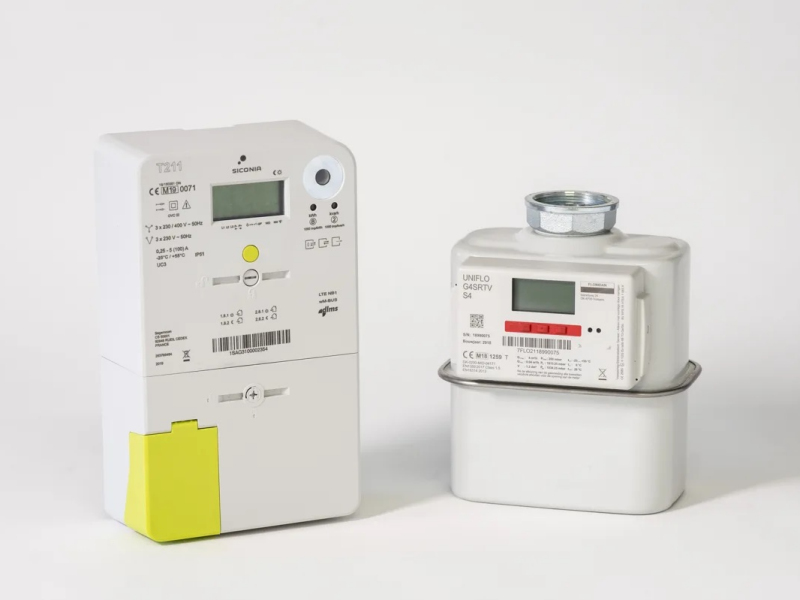
\includegraphics[width=0.9\textwidth]{SmartMeter.jpg}
  \caption{The new ''Smart Meter'' from Sagemcom}
\end{figure}

\eject


\chapter{Theory}


\section{The Smart Meter}

\subsection{Introduction}

The digital meters for electricity and gas were introduced in Flanders on 1 July 2019. Since then, they have replaced the old, mechanical meters that are no longer in circulation. Fluvius automatically installs them at new housing developments or renovations where the electricity connection is renewed. In addition, Fluvius launched a major geographical roll-out this spring to install such meters at every household and small business in Flanders. This will be organised by region, town or municipality. The roll-out aims at a complete conversion by 2029, with the main acceleration in the next three years. By the end of 2024, 80\% of homes should have digital meters.

\subsection{User-Ports}
These digital meters contain 2 User ports, which you are able to read you're consumption/production statistics from. The P1 port follows the DSMR 5 standard of the Dutch Smart Meter extended with the e-Mucs specification.
The S1 port provides a limited possibility of data and is going to be removed from the newer meters and is not going to be used in this project.
\subsection{Physical connection}

\begin{figure}[!ht]
    \centering
    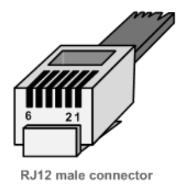
\includegraphics[width=3cm]{RJ12.png}
    \qquad
    \begin{tabular}{l|c} % <-- Alignments: 1st column left, 2nd middle with vertical lines in between
    \hline
      \textbf{Pin} & \textbf{Signal}\\
      \hline
      1 & 5V power supply\\
      2 & Data request (5V)\\
      3 & Data GND\\
      4 & Not connected\\
      5 & Data (open drain)\\
      6 & GND\\
    \end{tabular}
    \captionlistentry[table]{RJ12 connector and the pinout for the P1 port}
    \captionsetup{labelformat=andtable}
    \caption{RJ12 connector and the pinout for the P1 port}
  \end{figure}
  
\subsection{Internals of the meter}
\begin{figure}[H]
  \centering
  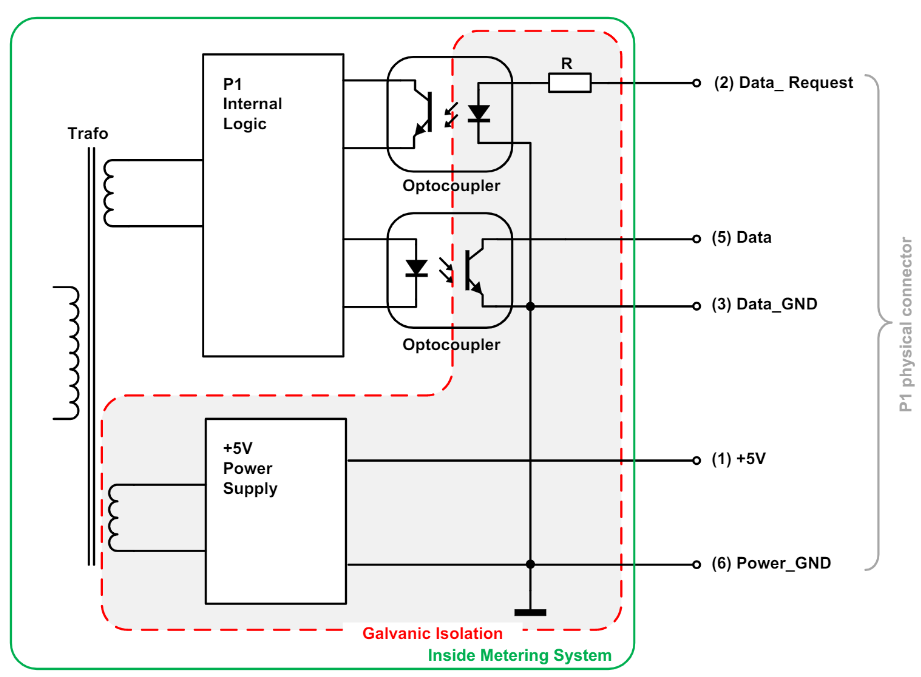
\includegraphics[width=0.9\textwidth]{MeterIntern.png}
  \caption{The internal workings of the Fluvius Meter}
\end{figure}
\subsubsection{+5V Power supply}
The P1 interface provides a stable +5V DC power supply via "+5V" (pin 1) and "GND"(pin 6) lines to provide a connected IoT device with a power source.

U = 5,0 V ( max = 5,5 V with I = 0 mA , min = 4,9 V with I = 250 mA )

\subsubsection{Data request}
The P1 port is activated (will start sending data) by setting "Data request" (pin 2) high (4,0V to 5,5V). While recieving data, this line must be kept high.

\textbf{Warning: To stop receiving data the "Data request" line must be put in a high impedance mode and must not be connected to the GND or 0V}

\subsubsection{Data}
Here we run into our first problem. Due to the use of optocouplers, the "Data" (pin 5) line must be designed as an Open Collector output and must be logically inverted or inverted via software before it can be used with IoT devices.

A "Data" line LOW has a voltage of 0,2 V (0 - 1V), HIGH has a voltage provided by a pull-up resistor to the VCC of the microcontroller with a maximum current of 30 mA.
For more information go to \url{https://www.netbeheernederland.nl/_upload/Files/Slimme_meter_15_a727fce1f1.pdf}
\vfill
\eject
\chapter{Project specifications}
\section{Components used}
\begin{itemize}
	\item ESP32-WROOM\tabto{11cm}(€5)
	\item Raspberry Pi/ PC\tabto{11cm}(Free)
	\item Waveshare e-paper display 3.7 inch 480x280px\tabto{11cm}(€42,13)
	\item extra components\tabto{11cm}(€20)
	
\end{itemize}

\section{Project Specifications}
The project is composed out of 3 parts: The sensor, the database and an observation unit. \ \\
The sensor side of the project contains all of the hardware that converts the data from the digital energy meter and sends that data to the database over WIFI once every couple of minutes (1-5 min).
\ \\
The database stores all of the records in a table. The data is received and send via a web-interface written in PHP and can be received via http requests. There will also be a dashboard that can be accessed via a web browser. But this is not important for this project.
\ \\
The display is the most important part of this project because it is the only visible part and has to be eye catching. It contains a graphical e-paper display to display the graph, a rotary encoder to select the data format (day, week, month or year) and you are able to ask for a specific format as example date format "week, -2" that will be two weeks prior to now.
\ \\
All of the parts are powered by a 5V wall adapter.


\begin{landscape}
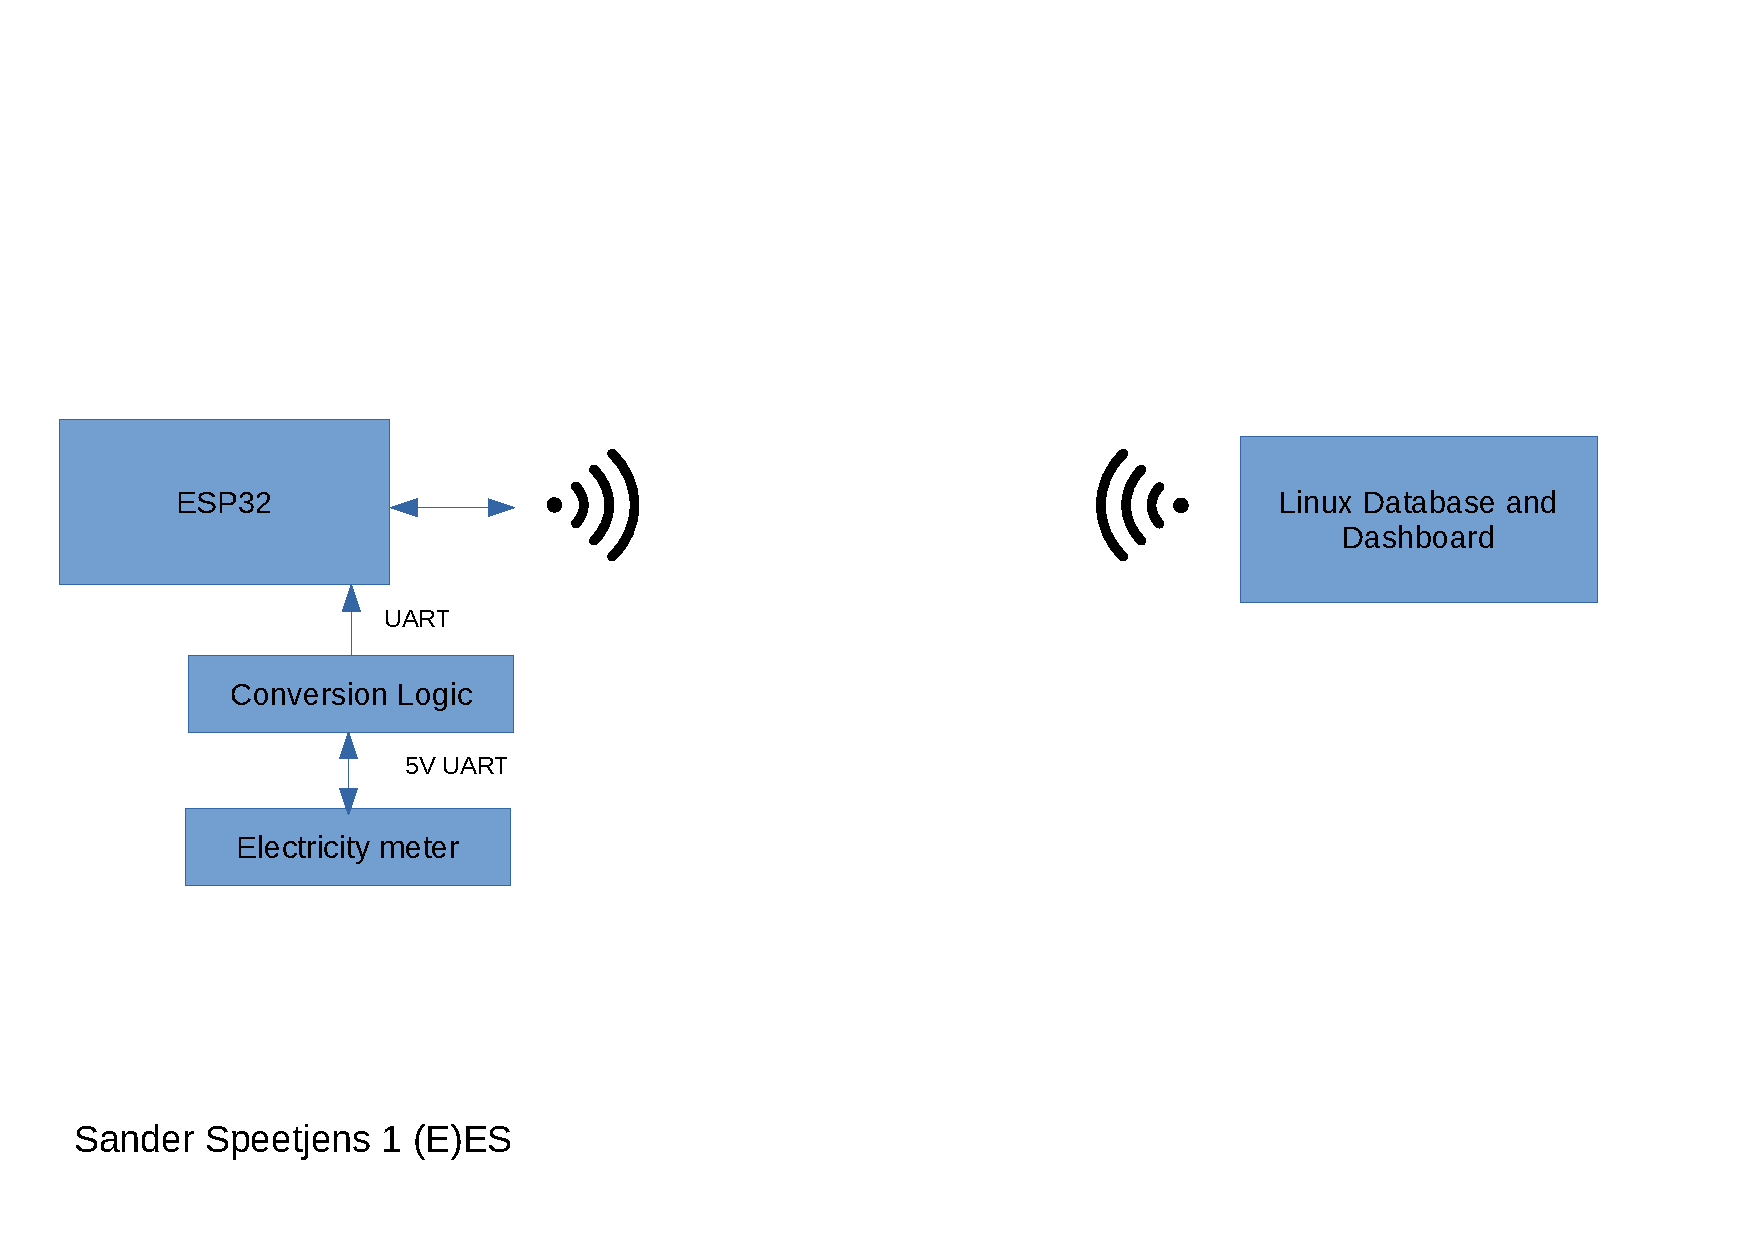
\includepdf[landscape=true, pagecommand=\section{Hardware Diagram}, pages=1]{Hardware.pdf}
\end{landscape}
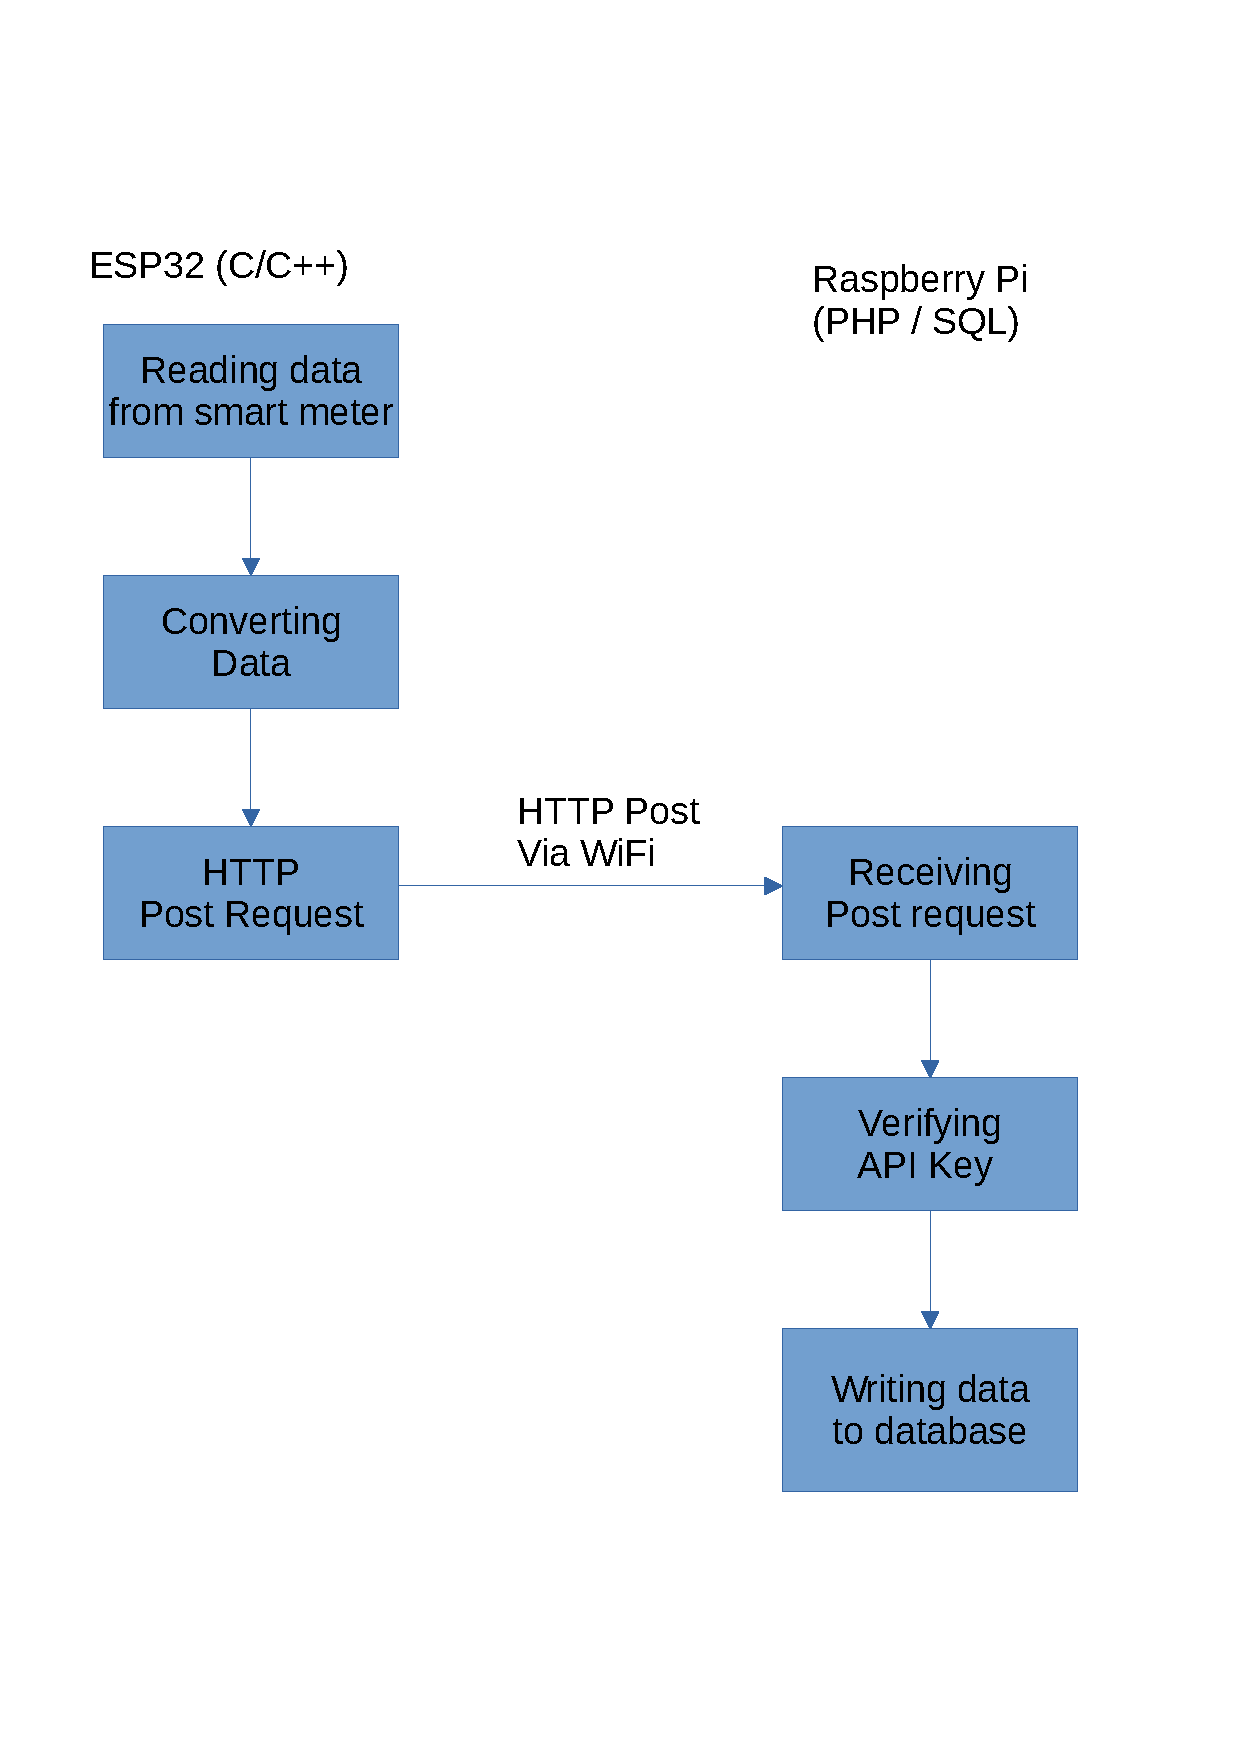
\includepdf[pagecommand=\section{Block diagram}, pages=-, scale=.95]{GIP-Blokschema-Programma.pdf}
\begin{landscape}
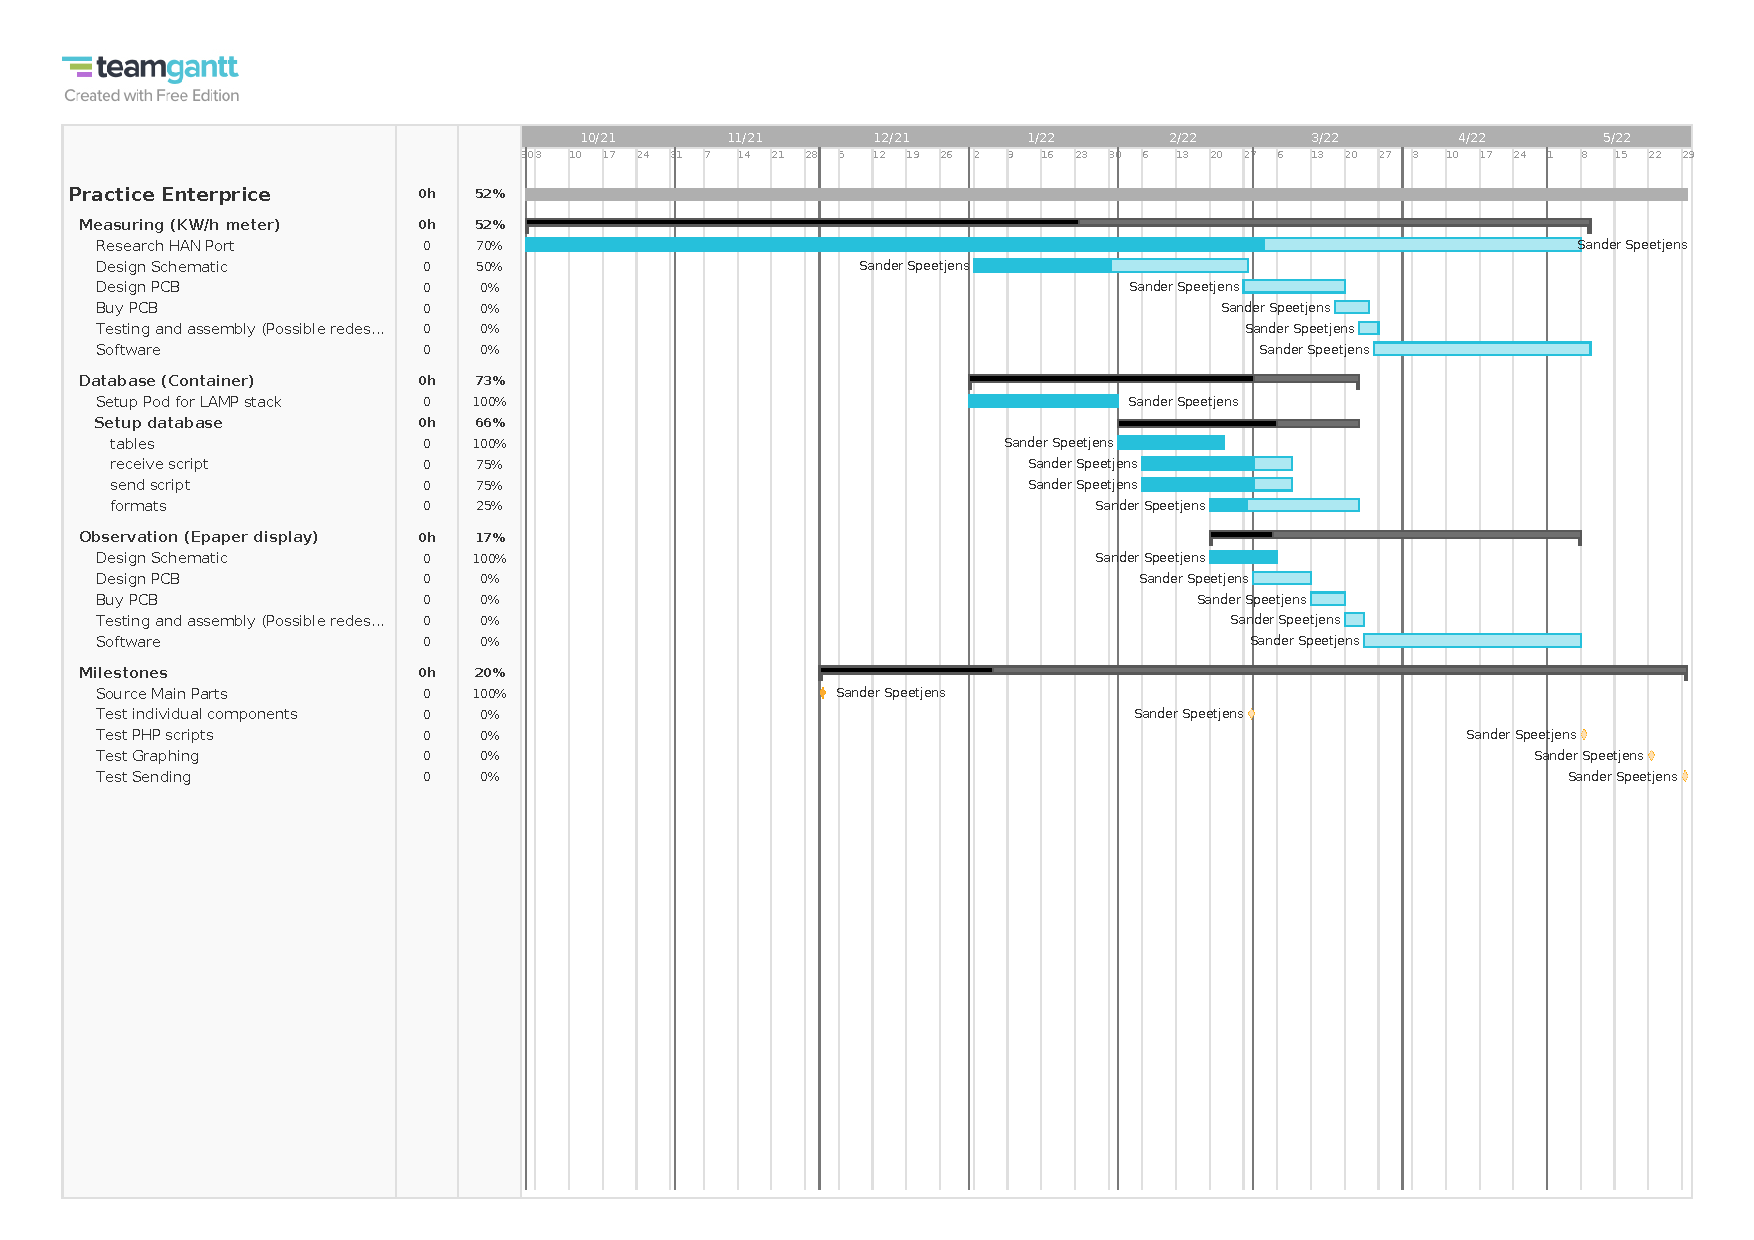
\includepdf[landscape=true, scale=.75, pagecommand=\section{Gantt Chart}, pages=1]{Gantt.pdf}
\end{landscape}

\end{document}